\documentclass[../main.tex]{subfiles}
\graphicspath{{\subfix{../images/}}}
\begin{document}
\subsection{Introduction To Probability}
\begin{definition}
A probability space is a 3-tuple $(\Omega,\mathcal{F},\mathbb{P})$ such that $\Omega\neq\emptyset$ (The sample space), $\mathcal{F}$ is a $\sigma-$algebra and $\mathbb{P}:\mathcal{F}\rightarrow [0,1]$ additive function. 
\end{definition}
\begin{definition} A $\sigma-$algebra $\mathcal{F}$ is a collection of sets over a set $\Omega$ such that - \\\\
(1). $\mathcal{F}\subseteq P(\Omega)$. \\\\
(2). $\Omega,\emptyset\in\mathcal{F}$. \\\\
(3). $\mathcal{F}$ is closed to the complements i.e. if $A\in\mathcal{F}$ then $A^C\in\mathcal{F}$. \\\\
(4). $\mathcal{F}$ is closed under countable union i.e. if $\{A_n\}_{n\in\mathbb{N}}\subset\mathcal{F}$ then $\bigcup_{n\in\mathbb{N}} A_n\in\mathcal{F}$. \\\\
The sets in $\mathcal{F}$ are called the measurable sets, the tuple $(\Omega,\mathcal{F})$ is called a measurable space. 
\end{definition}
\begin{definition} A function $\mathbb{P}:\mathcal{F}\rightarrow [0,1]$ over a measurable space $(\Omega,\mathcal{F})$ is a probability function if and only if the following happen: \\\\
(1). $\mathbb{P}(\emptyset) = 0,\mathbb{P}(\Omega) = 1$. \\\\
(2). For a collection of non-intersecting $\{A_n\}_{n\in\mathbb{N}}\subseteq \mathcal{F}$ we have:
\[\mathbb{P}(\biguplus_{n\in\mathbb{N}} A_n) = \sum_{n=1}^\infty \mathbb{P}(A_n)\]
\end{definition}
For countable sets $\Omega$ we usually take $\mathcal{F}:=2^{\Omega}$, the problem arises when we deal with non-countable sets where if we do take the power set to be the $\sigma$-algebra we get contradictions to the definition of the probability measure (for example take the Vitaly set). \\\\
Therefore when dealing, for example, with $\Omega:=[0,1]$ the normal way to define a probability space (with uniform probability) is to define for every interval $I\subseteq\Omega$ the probability to be it's length (in proportion to the original length which in this case is normalized to be 1). We can then take the $\sigma-$algebra to be the smallest one such that it contains every open interval in $\Omega$, this is called the Borel $\sigma-$algebra ($\mathcal{B}$).
\begin{definition} A function $X:\Omega\rightarrow\mathbb{R}$ such that for all $B\in\mathcal{B}$ we have $X^{-1}[B]\in\mathcal{F}$ is called measurable function, over a probability space it is called a random variable. \end{definition}
\begin{definition} Given a random variable X over a probability space $(\Omega,\mathcal{F},\mathbb{P})$ define a function $f_X:\mathbb{R}\rightarrow\mathbb{R}$ (the distribution) such that for all k we take $f_X(k) = \mathbb{P}(X=k)$. \end{definition}
\begin{definition} Given a random variable X over a probability space $(\Omega,\mathcal{F},\mathbb{P})$ define a function $F_X(r) = \mathbb{P}(X\leq r)$ (This is called the cumulative distribution function or the CDF). \end{definition}
\textbf{Characteristics Of A CDF:} 
\begin{itemize}
\item $F_X$ is monotone non-decreasing. 
\item $\lim_{x\rightarrow\infty} F_X(x) = 1.$ 
\item $\lim_{x\rightarrow-\infty} F_X(x) = 0.$
\item $F_X$ is continuous from the right. 
\end{itemize}
\begin{theorem}
If a function F satisfies the previous characteristics then there is a random variable X such that F is it's CDF. \end{theorem}
\begin{definition} For a random variable X with differentiable CDF $F_X$ If $F_X$ the density function $f_X$ is the derivative of $F_X$. \end{definition}
\textbf{Characteristics Of A Density Function:}\\\\
- For all $x\in\mathbb{R}$ we have $f(x)\geq 0$. \\\\
- $\int_{\mathbb{R}} f(x) dx = 1$. \\\\
\begin{theorem} Every integrable function with the previous characteristics is a density function for some random variable. \end{theorem}
\begin{definition} For $X,Y:\Omega\rightarrow \mathbb{R}$ random variables, we say that they are independent if and only if for all $A,B\in\mathcal{B}$ we have
\begin{center}
    $\mathbb{P}(X\in A\land Y\in B) = \mathbb{P}(X\in A)\cdot \mathbb{P}(Y\in B)$
\end{center}
Otherwise they are said to be dependent
\end{definition}
\newpage
\subsection{Important Discrete Distributions:}
\textbf{(1)}: Uniform Distribution - Given a finite set A we pick an element $a\in A$ with equal probability $\frac{1}{|A|}$ for every element. We denote $U[a,b]$ to be the uniform distribution on $\{a,a+1,\dots,b\}$. It's support is the set itself, and we have - 
\begin{center}
    $f_X(k):=\begin{cases} \frac{1}{b-a+1}, \text{ } a\leq k\leq b \\  0, \text{ Otherwise}\end{cases}$
\end{center}
\textbf{(2)}: Bernoulli Distribution with parameter p ($p\in[0,1]$). We say that $X\sim\text{Ber}(p)$ if 
\begin{center}
    $\mathbb{P}(X=r) = \begin{cases} p, \text{ } r=1 \\ 1-p, \text{ } r=0 \end{cases}$
\end{center} 
\textbf{(3)}: Binomial Distribution over n experiments and parameter p. We say that $X\sim\text{Bin}(n,p)$ if and only if for all $k\in\{0,1,\dots,n\}$ we have
\begin{center}
    $\mathbb{P}(X=k) = \binom{n}{k} p^k (1-p)^k$
\end{center}
\textbf{(4)}: The Geometric Distribution over $\mathbb{N}$ with parameter p. We say that $X\sim\text{Geo}(p)$ if and only if for all $k\in\mathbb{N}$ we have
\begin{center}
    $\mathbb{P}(X=k) = (1-p)^{k-1} p $
\end{center}
\textbf{(5)}: The Poisson Distribution over $\mathbb{N}$ with parameter $\lambda$. We say that $X\sim\text{Poi}(\lambda)$ if and only if for all $k\in\mathbb{N}$
\begin{center}
    $\mathbb{P}(X=k) = e^{-\lambda}\frac{\lambda^k}{k!}$
\end{center}
\newpage
\subsection{Important Uniform Distributions:}
\textbf{(1)}. Continuous Uniform Distribution over an interval $[a,b]\subset\mathbb{R}$. We say that $X\sim U[a,b]$ if it has the following characteristics \\
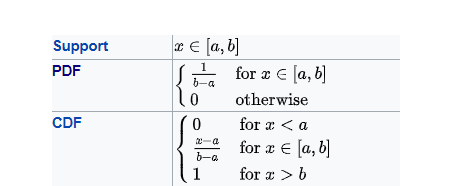
\includegraphics{images/Stat_Theory_First_Image.png}
\\
\textbf{(2)}. Exponential Distribution over $[0,\infty)$ with parameter $\lambda>0$. We say that $X\sim \text{Exp}(\lambda)$ if and only if it has the following characteristics \\\\
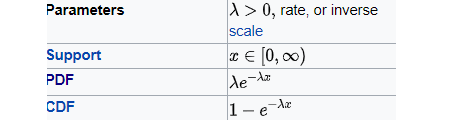
\includegraphics{images/Stat_Theory_Second_Image.png}
\\
\textbf{(3)}. Normal Distribution over $\mathbb{R}$ with parameters $\mu,\sigma$ ($\sigma>0$). We say that $X\sim \mathcal{N}(\mu,\sigma^2)$ if and only if it has the following characteristics \\\\
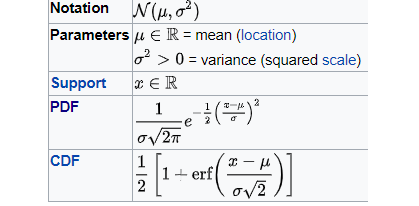
\includegraphics{images/Stat_Theory_Third_Picture.png}
\\
\newpage
\end{document}
